\begin{figure}[t]
    \centering
    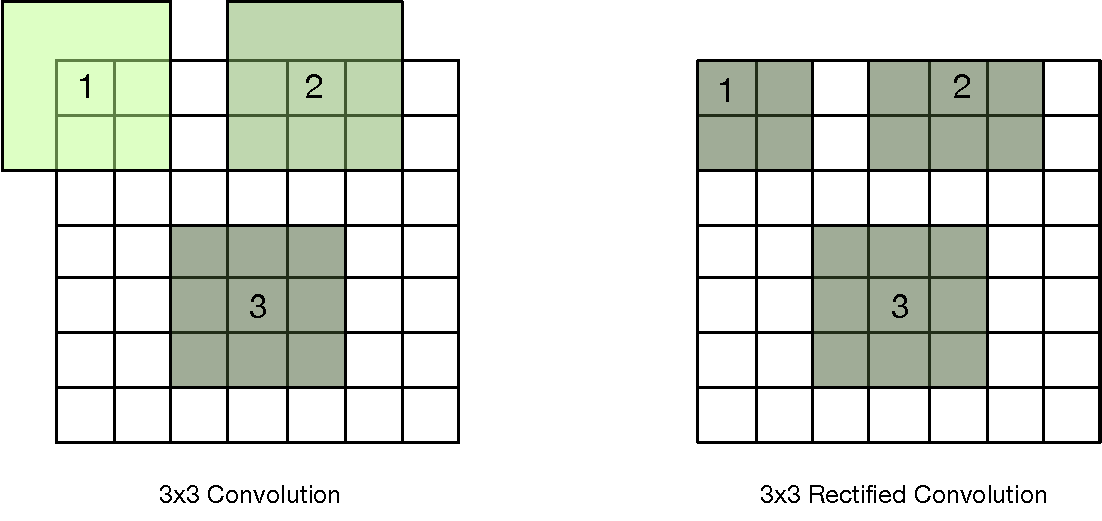
\includegraphics[width=0.9\linewidth]{fig/rectified_conv.pdf}
    \caption{Comparing to the standard 2D convolution with zero-padding, rectified convolution only takes the valid input values and scale up the activations based on number of valid input elements. The kernel size is $3\times 3$ and feature-map size is $7\times 7$. 
    %(Using different color to visualize the different number of valid pixels.)
    }
    \label{fig:rectified_conv}
\end{figure}